    \newcommand{\easymousefig}{
    \begin{figure}
        \centering
        \begin{subfigure}[t]{0.4\columnwidth}
            \centering
    \begin{tikzpicture}[scale=2]
        \draw[dashed](1,0)--(1.5,0);
        \node [fill=black,circle,minimum size=1pt,inner sep=0pt,outer sep=0pt] at (1.5,0) {} edge [in=50,out=130,loop,red] ();
    \end{tikzpicture}
    \caption{Case~\labelcref{case:newsl}}\label{fig:esl}
\end{subfigure}
\begin{subfigure}[t]{0.4\columnwidth}
    \centering
    \begin{tikzpicture}[scale=2]
    \draw[dashed](1,0)--(1.5,0);
    \draw[dashed] plot[smooth] coordinates{(1.5,0) (2,0.1) (2.4,0.04)};
    \draw[dashed] plot[smooth] coordinates{(1.5,0) (2,-0.1) (2.4,-0.04)};
    \draw[red,->] plot[smooth] coordinates{(2.4,0.04) (2.5,0)};
    \draw[red,->] plot[smooth] coordinates{(2.4,-0.04) (2.5,0)};
    \draw[dashed](1,0.2)--(2,0.2);
    \draw[red,->](2,0.2)--(2.1,0.2);
    \draw[dashed] plot[smooth] coordinates{(2.1,0.2) (2,0.3)(2.1,0.4) (2.2,0.3)};
    \draw[red,->] plot[smooth] coordinates{(2.2,0.3)(2.1,0.2)};
    \end{tikzpicture}
    \caption{Case~\labelcref{case:newcol}}\label{fig:encol}
\end{subfigure}
\begin{subfigure}[t]{0.4\columnwidth}
    \centering
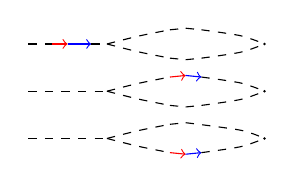
\begin{tikzpicture}[scale=2]
    \draw[dashed](1,0)--(1.5,0);
    \draw[dashed] plot[smooth] coordinates{(1.5,0) (1.7,0.05) (1.9,0.09)};
    \draw[dashed] plot[smooth] coordinates{(1.9,0.09) (2.0,0.1) };
    \draw[dashed] plot[smooth] coordinates{(2,0.1) (2.35,0.052) (2.5,0) };
    \draw[dashed] plot[smooth] coordinates{(1.5,0) (1.7,-0.05) (1.9,-0.09)};
    \draw[red,->] plot[smooth] coordinates{(1.9,-0.09) (2.0,-0.1) };
    \draw[blue,->] plot[smooth] coordinates{(2.0,-0.1) (2.1,-0.09) };
    \draw[dashed] plot[smooth] coordinates{(2.1,-0.09) (2.35,-0.052) (2.5,0) };


    \draw[dashed](1,0.3)--(1.5,0.3);
    \draw[dashed] plot[smooth] coordinates{(1.5,0.3) (1.7,0.35) (1.9,0.39)};
    \draw[red,->] plot[smooth] coordinates{(1.9,0.39) (2.0,0.4) };
    \draw[blue,->] plot[smooth] coordinates{(2,0.4) (2.1,0.39)};
    \draw[dashed] plot[smooth] coordinates{(2.1,0.39) (2.35,0.352) (2.5,0.3) };
    \draw[dashed] plot[smooth] coordinates{(1.5,0.3) (1.7,0.25) (1.9,0.21)};
    \draw[dashed] plot[smooth] coordinates{(1.9,0.21) (2.0,0.2) };
    \draw[dashed] plot[smooth] coordinates{(2.0,0.2) (2.1,0.21) };
    \draw[dashed] plot[smooth] coordinates{(2.1,0.21) (2.35,0.248) (2.5,0.3) };

    \draw[dashed](1,0.6)--(1.15,0.6);
    \draw[red,->](1.15,0.6)--(1.25,0.6);
    \draw[blue,->](1.25,0.6)--(1.4,0.6);
    \draw[dashed](1.4,0.6)--(1.5,0.6);
    \draw[dashed] plot[smooth] coordinates{(1.5,0.6) (1.7,0.65) (1.9,0.69)};
    \draw[dashed] plot[smooth] coordinates{(1.9,0.69) (2.0,0.7) };
    \draw[dashed] plot[smooth] coordinates{(2,0.7) (2.1,0.69)};
    \draw[dashed] plot[smooth] coordinates{(2.1,0.69) (2.35,0.652) (2.5,0.6) };
    \draw[dashed] plot[smooth] coordinates{(1.5,0.6) (1.7,0.55) (1.9,0.51)};
    \draw[dashed] plot[smooth] coordinates{(1.9,0.51) (2.0,0.5) };
    \draw[dashed] plot[smooth] coordinates{(2.0,0.5) (2.1,0.51) };
    \draw[dashed] plot[smooth] coordinates{(2.1,0.51) (2.35,0.548) (2.5,0.6) };
    \node [fill=black,circle,minimum size=1pt,inner sep=0pt,outer sep=0pt] at (2.5,0.6) () {};
    \node [fill=black,circle,minimum size=1pt,inner sep=0pt,outer sep=0pt] at (2.5,0.3) () {};
    \node [fill=black,circle,minimum size=1pt,inner sep=0pt,outer sep=0pt] at (2.5,0) () {};
% \draw[dashed](1,0.2)--(1.3,0.2);
% \draw[red,->](1.3,0.2)--(1.4,0.2);
% \draw[\repmcolor,->](1.4,0.2)--(1.5,0.2);
% \draw[dashed](1,0)--(1.3,0);
% \draw[red,->](1.3,0)--(1.4,0);
% \draw[blue,->](1.4,0)--(1.5,0);

\end{tikzpicture}
\caption{Case~\labelcref{case:repnew}}\label{fig:efa}
\end{subfigure}
\begin{subfigure}[t]{0.4\columnwidth}
    \centering
    \begin{tikzpicture}[scale=2]
        \draw[dashed](1,0)--(1.5,0);
        \node [fill=black,circle,minimum size=1pt,inner sep=0pt,outer sep=0pt] at (1.5,0) {} edge [in=50,out=130,loop,\repnmcolor] ();
    \end{tikzpicture}
    \caption{Case~\labelcref{case:oldsl}}\label{fig:eusl}
\end{subfigure}
\caption{Cases~\labelcref{case:newsl,case:newcol,case:repnew,case:oldsl}. The \new\ queries are drawn in {\color{red} red}, the \frep\ queries are drawn in {\color{\repmcolor} \repmcolor}, and the \urep\ queries are drawn in {\color{\repnmcolor}\repnmcolor}. The black dashed lines indicate zero or more queries of any type.}
\end{figure}
}

\newcommand{\unfammousefig}{
\begin{figure}
    \centering
    \begin{subfigure}[t]{0.42\columnwidth}
        \centering
    \begin{tikzpicture}[scale=3]
    \draw[dashed](1,0.6)--(1.5,0.6);
    \draw[dashed] plot[smooth] coordinates{(1.5,0.6) (2,0.7) (2.4,0.64)};
    \draw[dashed] plot[smooth] coordinates{(1.5,0.6) (1.9,0.51)};
    \draw[red,->](2.4,0.64)--node[above]{\color{red}$q_2$}(2.5,0.6);
    \draw[red,->](1.9,0.51)--node[below]{\color{red}$q_1$}(2.0,0.5);
    \draw[dashed,\repnmcolor] plot[smooth] coordinates{(2,0.5) (2.35,0.548) (2.4,0.56) };
    \draw[\repnmcolor,->](2.4,0.56)--node[below]{\color{\repnmcolor}$q_3$}(2.5,0.6);
    
    
    \draw[dashed](1,0.9)--(1.6,0.9);
    \draw[red,->](1.6,0.9)--node[midway,below]{\color{red}$q_1$}(1.7,0.9);
    \draw[dashed,\repnmcolor](1.7,0.9)--(2,0.9);
        \draw[\repnmcolor,->](2,0.9)--node[midway,below]{\color{\repnmcolor}$q_3$}(2.1,0.9);
        \draw[dashed] plot[smooth] coordinates{(2.1,0.9) (2,1)(2.1,1.1) (2.2,1)};
        \draw[red,->] (2.2,1)--node[below]{\color{red}$q_2$}(2.1,0.9);
        \draw[dashed,black](1,1.3)--(2,1.3);
        \draw[red,->](2,1.3)--node[below]{\color{red}$q_2$}(2.1,1.3);
        \draw[dashed,black] plot[smooth] coordinates{(2.1,1.3) (2,1.4)};
        \draw[red,->] (2,1.4)--node[midway,above]{\color{red}$q_1$}(2.1,1.5) ;
        \draw[dashed,\repnmcolor] plot[smooth] coordinates{(2.1,1.5) (2.2,1.4)};
        \draw[\repnmcolor,->] (2.2,1.4)--node[midway,below]{\color{\repnmcolor}$q_3$}(2.1,1.3);


        \draw[dashed](1,0.3)--(1.2,0.3);
        \draw[->,red](1.2,0.3)--node[below]{\color{red}$q_1$}(1.3,0.3);
        \draw[dashed,\repnmcolor](1.3,0.3)--(1.5,0.3);
        \draw[dashed] plot[smooth] coordinates{(1.5,0.3) (2,0.4) (2.4,0.34)};
        \draw[dashed,\repnmcolor] plot[smooth] coordinates{(1.5,0.3) (1.9,0.21)};
        \draw[red,->](2.4,0.34)--node[above]{\color{red}$q_2$}(2.5,0.3);
        \draw[dashed,\repnmcolor](1.9,0.21)--(2.0,0.2);
        \draw[dashed,\repnmcolor] plot[smooth] coordinates{(2,0.2) (2.35,0.248) (2.4,0.26) };
        \draw[\repnmcolor,->](2.4,0.26)--node[below]{\color{\repnmcolor}$q_3$}(2.5,0.3);
        

    \end{tikzpicture}
    \caption{Mouse structures with at least one \new\ query in their body and a \new\ query at the tip}\label{fig:newsixtip} 
\end{subfigure}\hfill
\begin{subfigure}[t]{0.42\columnwidth}
    \centering
\begin{tikzpicture}[scale=3]
\draw[dashed](1,0)--(1.5,0);
\draw[dashed] plot[smooth] coordinates{(1.5,0) (1.7,0.05) (1.9,0.09)};
\draw[red,->] (1.9,0.09)--node[above]{\color{red}$q_1$}(2.0,0.1) ;
\draw[dashed,\repnmcolor] plot[smooth] coordinates{(2,0.1) (2.35,0.052) (2.4,0.04) };
\draw[dashed] plot[smooth] coordinates{(1.5,0) (1.7,-0.05) (1.9,-0.09)};
\draw[red,->] (1.9,-0.09) --node[below]{\color{red}$q_2$}(2.0,-0.1) ;
\draw[dashed,\repnmcolor] plot[smooth] coordinates{(2,-0.1) (2.35,-0.052) (2.4,-0.04) };
\draw[\repnmcolor,->] (2.4,0.04)--node[above]{\color{\repnmcolor}$q_3$}(2.5,0);
\draw[\repnmcolor,->] (2.4,-0.04)--node[below]{\color{\repnmcolor}$q_4$}(2.5,0);


\draw[dashed](1,0.3)--(1.5,0.3);
\draw[red,->] (1.5,0.3)--node[below]{\color{red}$q_1$}(1.6,0.3);
\draw[\repnmcolor,dashed](1.6,0.3)--(2,0.3);
\draw[\repnmcolor,->](2,0.3)--node[below]{\color{\repnmcolor}$q_3$}(2.1,0.3);
\draw[dashed] plot[smooth] coordinates{(2.1,0.3) (2,0.4)};
\draw[\repnmcolor,dashed] plot[smooth] coordinates{(2.1,0.5)(2.2,0.4) };
\draw[red,->] (2,0.4)--node[above]{\color{red}$q_2$}(2.1,0.5) ;
\draw[\repnmcolor,->](2.2,0.4)--node[below]{\color{\repnmcolor}$q_4$}(2.1,0.3);



\draw[dashed](1,-0.3)--(1.2,-0.3);
\draw[red,->](1.2,-0.3)--node[below]{\color{red}$q_1$}(1.3,-0.3);
\draw[dashed,\repnmcolor](1.3,-0.3)--(1.5,-0.3);
\draw[dashed,\repnmcolor] plot[smooth] coordinates{(1.5,-0.3) (1.7,-0.25) (1.9,-0.21)};
\draw[dashed,\repnmcolor] (1.9,-0.21)--(2.0,-0.2) ;
\draw[dashed,\repnmcolor] plot[smooth] coordinates{(2,-0.2) (2.35,-0.248) (2.4,-0.26) };
\draw[dashed] plot[smooth] coordinates{(1.5,-0.3) (1.7,-0.35) (1.9,-0.39)};
\draw[red,->] (1.9,-0.39) --node[below]{\color{red}$q_2$}(2.0,-0.4) ;
\draw[dashed,\repnmcolor] plot[smooth] coordinates{(2,-0.4) (2.35,-0.352) (2.4,-0.34) };
\draw[\repnmcolor,->] (2.4,-0.26)--node[above]{\color{\repnmcolor}$q_3$}(2.5,-0.3);
\draw[\repnmcolor,->] (2.4,-0.34)--node[below]{\color{\repnmcolor}$q_4$}(2.5,-0.3);

\end{tikzpicture}
\caption{Mouse structures with at least one \new\ query in their body and no \new\ query at the tip}\label{fig:newsixnotip} 
\end{subfigure}\\
    \begin{subfigure}[t]{0.42\columnwidth}
        \centering
    \begin{tikzpicture}[scale=3]
        %     \draw[dashed](1,0)--(1.3,0);
        %     \draw[red, ->](1.3,0)--(1.4,0);
        %     \draw[dashed,\repnmcolor](1.4,0)--(1.5,0);
        %     \draw[dashed,\repnmcolor] plot[smooth] coordinates{(1.5,0) (2,0.1) (2.4,0.04)};
        %     \draw[dashed,\repnmcolor] plot[smooth] coordinates{(1.5,0) (2,-0.1) (2.4,-0.04)};
        %     \draw[\repnmcolor,->] plot[smooth] coordinates{(2.4,0.04) (2.5,0)};
        %     \draw[\repnmcolor,->] plot[smooth] coordinates{(2.4,-0.04) (2.5,0)};
    
    
        %     \draw[dashed](1,0.3)--(1.5,0.3);
        % \draw[red,->] (1.5,0.3)--(1.6,0.3);
        % \draw[\repnmcolor,dashed](1.6,0.3)--(2,0.3);
        % \draw[\repnmcolor,->](2,0.3)--(2.1,0.3);
        % \draw[\repnmcolor,dashed] plot[smooth] coordinates{(2.1,0.3) (2,0.4)(2.1,0.5) (2.2,0.4)};
        % \draw[\repnmcolor,->] plot[smooth] coordinates{(2.2,0.4)(2.1,0.3)};
   
    
        \draw[dashed](1,0)--(1.5,0);
        \draw[red,->](1.5,0)--node[below]{\color{red}$q_1$}(1.6,0);
        \draw[\repnmcolor,dashed](1.6,0)--(2.1,0);
        \draw[\repnmcolor,->] (2.1,0) --node[above]{\color{\repnmcolor}$q_2$}(2,0.1);
        \draw[dashed,\repnmcolor] plot[smooth] coordinates{(2,0.1)(2.1,0.2) (2.2,0.1)};
        \draw[\repnmcolor,->] (2.2,0.1)--node[below]{\color{\repnmcolor}$q_3$}(2.1,0);
    \end{tikzpicture}
\caption{Mouse structure with no \new\ query in the body, and the body of the mouse structure is a directed cycle}\label{fig:nonewsixtip} 
   \end{subfigure}\hfill
    \begin{subfigure}[t]{0.42\columnwidth}
        \centering
        \begin{tikzpicture}[scale=3]
        \draw[dashed](1,0)--(1.3,0);
        \draw[red, ->](1.3,0)--node[below]{\color{red}$q_1$}(1.4,0);
        \draw[dashed,\repnmcolor](1.4,0)--(1.5,0);
        \draw[dashed,\repnmcolor] plot[smooth] coordinates{(1.5,0) (2,0.1) (2.4,0.04)};
        \draw[dashed,\repnmcolor] plot[smooth] coordinates{(1.5,0) (2,-0.1) (2.4,-0.04)};
        \draw[\repnmcolor,->] (2.4,0.04)--node[above]{\color{\repnmcolor}$q_2$}(2.5,0);
        \draw[\repnmcolor,->] (2.4,-0.04)--node[below]{\color{\repnmcolor}$q_3$}(2.5,0);


    %     \draw[dashed](1,0.3)--(1.5,0.3);
    % \draw[red,->] (1.5,0.3)--node[below]{\color{red}$q_1$}(1.6,0.3);
    % \draw[\repnmcolor,dashed](1.6,0.3)--(2,0.3);
    % \draw[\repnmcolor,->](2,0.3)--node[below]{\color{\repnmcolor}$q_2$}(2.1,0.3);
    % \draw[\repnmcolor,dashed] plot[smooth] coordinates{(2.1,0.3) (2,0.4)(2.1,0.5) (2.2,0.4)};
    % \draw[\repnmcolor,->] (2.2,0.4)--node[below]{\color{\repnmcolor}$q_3$}(2.1,0.3);
        \end{tikzpicture}
    \caption{Mouse structure with no \new\ query in the body, but the body of the mouse structure is not a directed cycle}\label{fig:nonewsixnotip}        
\end{subfigure}


\caption{Mouse structures categorized in case~\labelcref{case:norep}. The \new\ queries are drawn in {\color{red} red}, and the \urep\ queries are drawn in {\color{\repnmcolor}\repnmcolor}. The black dashed lines indicate zero or more \new\ or \urep\ queries.}\label{fig:unfam}
\end{figure}
}
\newcommand{\fammousefig}{
\begin{figure}
    \centering
    
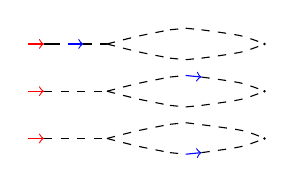
\begin{tikzpicture}[scale=2]
    \draw[red,->](1,0)--(1.1,0);
    \draw[dashed](1.1,0)--(1.5,0);
    \draw[dashed] plot[smooth] coordinates{(1.5,0) (1.7,0.05) (1.9,0.09)};
    \draw[dashed] plot[smooth] coordinates{(1.9,0.09) (2.0,0.1) };
    \draw[dashed] plot[smooth] coordinates{(2,0.1) (2.35,0.052) (2.5,0) };
    \draw[dashed] plot[smooth] coordinates{(1.5,0) (1.7,-0.05) (1.9,-0.09)};
    \draw[dashed] plot[smooth] coordinates{(1.9,-0.09) (2.0,-0.1) };
    \draw[blue,->] plot[smooth] coordinates{(2.0,-0.1) (2.1,-0.09) };
    \draw[dashed] plot[smooth] coordinates{(2.1,-0.09) (2.35,-0.052) (2.5,0) };
    \node [fill=black,circle,minimum size=1pt,inner sep=0pt,outer sep=0pt] at (2.5,0) () {};

    \draw[red,->](1,0.3)--(1.1,0.3);
    \draw[dashed](1.1,0.3)--(1.5,0.3);
    \draw[dashed] plot[smooth] coordinates{(1.5,0.3) (1.7,0.35) (1.9,0.39)};
    \draw[dashed] plot[smooth] coordinates{(1.9,0.39) (2.0,0.4) };
    \draw[blue,->] plot[smooth] coordinates{(2,0.4) (2.1,0.39)};
    \draw[dashed] plot[smooth] coordinates{(2.1,0.39) (2.35,0.352) (2.5,0.3) };
    \draw[dashed] plot[smooth] coordinates{(1.5,0.3) (1.7,0.25) (1.9,0.21)};
    \draw[dashed] plot[smooth] coordinates{(1.9,0.21) (2.0,0.2) };
    \draw[dashed] plot[smooth] coordinates{(2.0,0.2) (2.1,0.21) };
    \draw[dashed] plot[smooth] coordinates{(2.1,0.21) (2.35,0.248) (2.5,0.3) };
    \node [fill=black,circle,minimum size=1pt,inner sep=0pt,outer sep=0pt] at (2.5,0.3) () {};

    \draw[red,->](1,0.6)--(1.1,0.6);
    \draw[dashed](1.1,0.6)--(1.15,0.6);
    \draw[dashed](1.15,0.6)--(1.25,0.6);
    \draw[blue,->](1.25,0.6)--(1.35,0.6);
    \draw[dashed](1.35,0.6)--(1.5,0.6);
    \draw[dashed] plot[smooth] coordinates{(1.5,0.6) (1.7,0.65) (1.9,0.69)};
    \draw[dashed] plot[smooth] coordinates{(1.9,0.69) (2.0,0.7) };
    \draw[dashed] plot[smooth] coordinates{(2,0.7) (2.1,0.69)};
    \draw[dashed] plot[smooth] coordinates{(2.1,0.69) (2.35,0.652) (2.5,0.6) };
    \draw[dashed] plot[smooth] coordinates{(1.5,0.6) (1.7,0.55) (1.9,0.51)};
    \draw[dashed] plot[smooth] coordinates{(1.9,0.51) (2.0,0.5) };
    \draw[dashed] plot[smooth] coordinates{(2.0,0.5) (2.1,0.51) };
    \draw[dashed] plot[smooth] coordinates{(2.1,0.51) (2.35,0.548) (2.5,0.6) };
    \node [fill=black,circle,minimum size=1pt,inner sep=0pt,outer sep=0pt] at (2.5,0.6) () {};


\end{tikzpicture}
\caption{Mouse structure for case~\labelcref{case:somerep}}\label{fig:fammouse}
\end{figure}
}


\newcommand{\ovhardcasefig}{
\begin{figure}[t]
    \centering
    
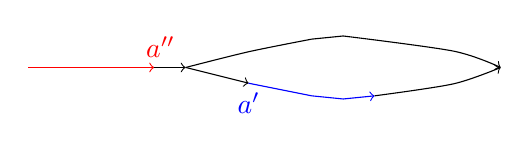
\begin{tikzpicture}[scale=4]
    \draw[red,->](1.0,0)--(1.4,0);
    \node [above] at (1.42,0) () {{\color{red}{$a''$}}};
    \node [fill=red,circle,minimum size=0.2pt,inner sep=0pt,outer sep=0pt] at (1.4,0) () {};
    \draw[\repnmcolor,->](1.4,0)--(1.5,0);
    \draw[\repnmcolor] plot[smooth] coordinates{(1.5,0) (1.7,0.05) (1.9,0.09)};
    \draw[\repnmcolor] plot[smooth] coordinates{(1.9,0.09) (2.0,0.1) };
    \draw[\repnmcolor,->] plot[smooth] coordinates{(2,0.1) (2.35,0.052) (2.5,0) };
    \draw[\repnmcolor,->] plot[smooth] coordinates{(1.5,0) (1.7,-0.05) };
    \node [below] at (1.7,-0.05) () {{\color{blue}{$a'$}}};
    \node [fill=blue,circle,minimum size=0.2pt,inner sep=0pt,outer sep=0pt] at (1.7,-0.05) () {};
    \draw[blue] plot[smooth] coordinates{(1.7,-0.05) (1.9,-0.09)};
    \draw[blue] plot[smooth] coordinates{(1.9,-0.09) (2.0,-0.1) };
    \draw[blue,->] plot[smooth] coordinates{(2.0,-0.1) (2.1,-0.09) };
    \draw[\repnmcolor,->] plot[smooth] coordinates{(2.1,-0.09) (2.35,-0.052) (2.5,0) };
    

\end{tikzpicture}
\caption{An example of a ``hard'' mouse structure. The \new\ queries are drawn in {\color{red} red}, \frep\ queries are drawn in {\color{blue} blue} and the \urep\ queries are drawn in {\color{\repnmcolor}\repnmcolor}.}\label{fig:hardcaseto}
\end{figure}
}






\newcommand{\mulcolfig}{
\begin{figure}
    \centering
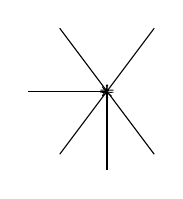
\begin{tikzpicture}[scale=1]
    \draw[->](-1,0.0)--(0,0.0);
    \draw[->](0.0,-1)--(0,0.0);
    \draw[->](0.6,0.8)--(0,0.0);
    \draw[->](0.6,-0.8)--(0,0.0);
    \draw[->](-0.6,0.8)--(0,0.0);
    \draw[->](-0.6,-0.8)--(0,0.0);
\end{tikzpicture}
\caption{Multi-collisions}\label{fig:mulcol}
\end{figure}
}

\newcommand{\encodetree}{
\tikzset{
  treenode/.style = {shape=rectangle, rounded corners,
                     draw, align=center,
                     top color=white, bottom color=blue!20},
  root/.style     = {treenode, font=\Large, bottom color=red!30},
  env/.style      = {treenode, font=\ttfamily\normalsize},
  dummy/.style    = {circle,draw}
}
\begin{figure}
    \centering
\begin{tikzpicture}
    [
      grow                    = down,
      level 1/.style={sibling distance=18em,level distance = 10em},
  level 2/.style={sibling distance=12em,level distance = 10em},
  level 3/.style={sibling distance=6em,level distance = 12em},
  level 4/.style={sibling distance=6em,level distance = 14em},
      edge from parent/.style = {draw, -latex},
      every node/.style       = {font=\scriptsize},
      sloped
    ]
    \node [root] {Mouse structure}
    child { node [dummy] {}
    child { node [env] {$\esl$}
      edge from parent node [above] {new self-loop} }
      child { node [env,left=3em] {$\encol$}
      edge from parent node [above] {new collision} }
      child { node [env,left=8em] {$\efc$}
      edge from parent node [above] {familiar collision} }
      child { node [env,left=12em] {$\eul$}
      edge from parent node [above] {unfamiliar self-loop} }
            edge from parent node [above] {easy} }
    child { node [dummy,left=3em] {}
    child { node [dummy] {}
    child { node [dummy] {}
    child { node [env] {$\guosn$}
      edge from parent node [above] {common source newer tip} }
      child { node [env] {$\gutsn$}
      edge from parent node [above] {distinct sources newer tip} }
      child { node [env] {$\guoso$}
      edge from parent node [above] {common source older tip} }
      child { node [env] {$\gutso$}
      edge from parent node [above] {distinct sources older tip} }
      edge from parent node [above] {unused paths} }
      child { node [env] {$\gf$}
        edge from parent node [above] {used path} }
      edge from parent node [above] {good} }
      child { node [dummy] {}
    child { node [env] {$\mc$}
      edge from parent node [above] {Unrecorded} }
      child { node [env] {$\smc$}
      edge from parent node [above] {Semi-recorded} }
      child { node [dummy] {}
      edge from parent node [above] {Recorded} }
      edge from parent node [above] {bad} }
            edge from parent node [above] {difficult} };
  \end{tikzpicture}
  \caption{Graphical representation of the encoding algorithm. The leaf nodes are the subroutines defined earlier. If the mouse structure is difficult, bad and has a recorded multi-collision we do nothing.}\label{fig:enctree}
\end{figure}
}